\documentclass[11pt]{article}
\usepackage[margin=1in]{geometry}
\usepackage{amsmath,amsthm,amssymb}
\usepackage{graphicx}

\title{New Methods for Studying Old Work}
\author{José Ignacio Velarde Morales}

\begin{document}
\maketitle
\tableofcontents

\section{Introduction}
  \subsection{Motivation for studying new work}
  \subsection{ML for econ}

\section{Related Literature}
  \subsection{Literature about new work}
  \subsection{NLP literature}
  \subsection{Econ and ML literature}

\section{Data}
  \subsection{Dictionary of Occupational Titles}
  The Dictionary of Occupational Titles (DOT) is a volume that was created by the United States Department of Labor to help match job openings and job seekers. It provides detailed textual descriptions of thousands of jobs. The job descriptions generally describe what work is done, who it is done by, and why it is done. The descriptions also include information regarding the industry and occupation group the job is in.

  \begin{figure}[h]
    \centering
    \caption{Example definition from the 1939 DOT}
    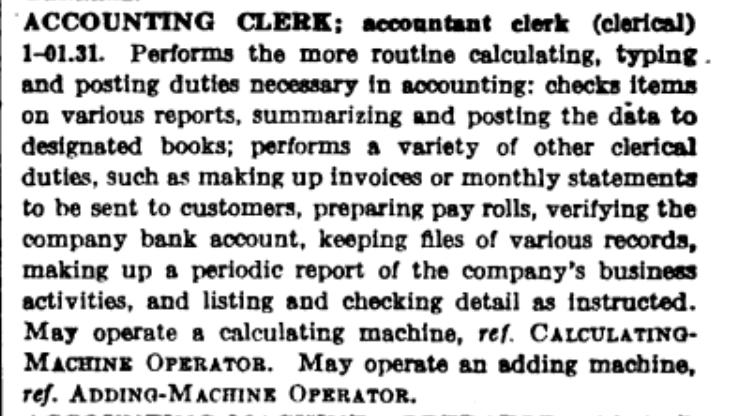
\includegraphics[width=0.6\textwidth, keepaspectratio=true]{images/dot_def}
  \end{figure}

  There are 5 editions of the DOT, published in 1939, 1949, 1965, 1977, and 1991. Each edition has about 20,000 job definitions. The 1965, 1977, and 1991 editions of the DOT include structured information about the jobs in addition to the textual description. The structured information is in the form of numerical codes that quantify job complexity, training requirements, and skill requirements. These codes are further described below.

  \subsubsection*{Data, People, Things Codes}
  Each job is assigned a 3-digit code that describes the job's complexity in relation to data, people, and things. Each digit in the code corresponds the job's complexity in one of those three categories. For example, the job of Aeronautical Test Engineer has a code of 061. The code tells us the job has high data complexity, medium/low people complexity, and high things complexity. The figure below shows the meanings of the different codes.

      \begin{figure}[h]
        \centering
        \caption{Explanation of Data, People, Things Code}
        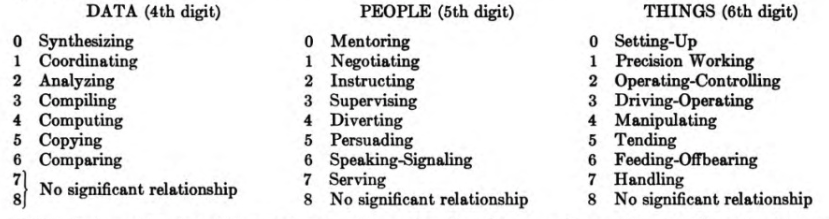
\includegraphics[width=0.95\textwidth, keepaspectratio=true]{images/DPT}
      \end{figure}

  \subsubsection*{Job Attributes}
  Job descriptions in the DOT include descriptions of the mathematical education, aptitudes, and temperaments required to perform each job. Mathematical education refers to formal and informal education that develops basic reasoning skills in math. Aptitudes are specific abilities that an individual should have in order to perform a specific job. Examples of aptitudes are finger dexterity and hand-eye coordination. Temperaments are adaptability requirements made on the worker by specific types of job situations. These can include directing activities or performing repetitive work. The full list of job attributes we predict can be found in the table below.
  % TODO: improve attributes description.

    \begin{table}[h!]
      \centering
      \begin{tabular}{|l|l|l|}
      \hline
      \textbf{Attribute}         & \textbf{Description}                                                   & \textbf{Scale} \\ \hline
      GED Math                   & Formal and informal education developing general math skills           & 1-6            \\ \hline
      Finger Dexterity           & Ability to use fingers to manipulate small objects                     & 1-5            \\ \hline
      Eye-hand-foot Coordination & Motor responsiveness to visual stimuli                                 & 1-5            \\ \hline
      Direct, control, plan      & Situations involving the direction, control and planning of activities & 0/1            \\ \hline
      Attain limits              & Situations involving the precise attainment of set limits or standards & 0/1            \\ \hline
      \end{tabular}
    \end{table}


  \subsection{1940 Census Complete Count Files}
  The United States conducts a census every ten years to collect data about its population. The Census collects a wide range of information about respondents including occupation, income, education, and place of residence. The data is confidential, but becomes publicly available 72 years after Census Day. The data from the 1940 Census became publicly available in April of 2012.
  % Add stuff about micro data vs CCC, and occupation codes

  \subsection{CAI}

\section{Methods}
  \subsection{Methods used}
    \subsubsection{TF-IDF}
    \subsubsection{RoBERTa}

  \subsection{Matching procedure}

  \subsection{Prediction}

\section{Results}
  \subsection{Matching Rate/Validation}
  \subsection{Attribute Prediction}

\section{Conclusion}








\end{document}
